\documentclass[10pt, a4paper]{article}
\usepackage[utf8]{inputenc}
\usepackage[spanish]{babel}

\usepackage{varwidth}
\usepackage{graphicx}
\usepackage{eurosym} % para el euro

\usepackage[T1]{fontenc} % Use 8-bit encoding that has 256 glyphs


\usepackage[hmarginratio=1:1,top=32mm,columnsep=20pt]{geometry} % Document margins
\usepackage[hang, small,labelfont=bf,up,textfont=it,up]{caption} % Custom captions under/above floats in tables or figures

\usepackage{float} % Required for tables and figures in the multi-column environment - they need to be placed in specific locations with the [H] (e.g. \begin{table}[H])

\usepackage{hyperref} % For hyperlinks in the PDF


\usepackage{amsmath,amssymb}


\usepackage{titlesec} % Allows customization of titles
\renewcommand\thesection{} % Roman numerals for the sections
\renewcommand\thesubsection{\alph{subsection}} % Roman numerals for subsections
\titleformat{\section}[block]{\large\scshape\centering}{\thesection}{1em}{} % Change the look of the section titles
\titleformat{\subsection}[block]{\large}{\thesubsection.}{1em}{} % Change the look of the section titles

\usepackage{fancyhdr} % Headers and footers
\pagestyle{fancy} % All pages have headers and footers
\fancyhead{} % Blank out the default header
\fancyfoot{} % Blank out the default footer
\fancyhead[C]{Sergio García Prado $\bullet$ Marzo 2016 $\bullet$ Modelos para la Toma de Decisiones $\bullet$ Tarea 1} % Custom header text
\fancyfoot[RO,LE]{\thepage} % Custom footer text

%----------------------------------------------------------------------------------------
%	TITLE SECTION
%----------------------------------------------------------------------------------------

\title{\vspace{-15mm}\fontsize{24pt}{10pt}\selectfont\textbf{Modelos para la Toma de Decisiones: Tarea 1}} % Article title

\author{
\large
\textsc{Sergio García Prado}\\[2mm] % Your name
\normalsize Universidad de Valladolid \\ % Your institution
\vspace{-5mm}
}
\date{}

%----------------------------------------------------------------------------------------

\begin{document}

	\maketitle % Insert title

	\thispagestyle{fancy} % All pages have headers and footers

%----------------------------------------------------------------------------------------
%	TEXT
%----------------------------------------------------------------------------------------

    \section{Ejercicio 1}

        \begin{figure}[H]
        \centering
            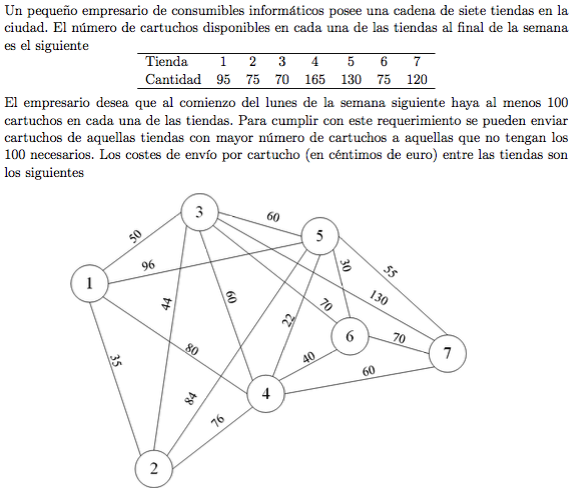
\includegraphics[width=0.75\textwidth]{res/Exercise_1.png}
        \end{figure}

		\subsection{Determinar la mejor manera de distribuir los cartuchos entre las tiendas.}

			\paragraph{}
			Lo primero que haremos será modelar el enunciado del problema. Se ha tenido en cuenta el detalle que indica que los envíos de cartuchos tan solo son posibles desde las tiendas que tienen un exceso de cartuchos (más de 100) a las que tienen déficit (menos de 100).

			\paragraph{}
			La notación que se va a utilizar para denotar las variables es la siguiente:
			\paragraph{}
			\(x_{ij}\) = Número de cartuchos enviados desde la tienda \(i\) hasta la tienda \(j\). \(\quad i=4,5,7. \quad j=1,2,3,6.\)

			\paragraph{}
			Notese que tal y como indica el enunciado del problema la función objetivo de este consistirá en minimizar la suma de costes necesarios para llegar al objetivo del número de cartuchos por tienda. Por tanto las restricciones asociadas al problema servirán para restringir el tanto el número de cartuchos que se pueden envíar a partir de una tienda de origen, como el número necesario de cartuchos que se necesitan en el caso de las tiendas de destino.

			\paragraph{}
			A continuación se muestra la modelización del problema:

			\[
			  \begin{array}{r@{}r@{}r@{}r@{}r@{}r@{}r@{}r@{}r@{}r@{}l}
			    \text{Min} \quad z=	80x_{41} &{} + 76x_{42} &{} + 60x_{43} &{} + 40x_{46} &{} + 96x_{51} &{} + 84x_{52} &{} + 60x_{53} &{} + 30x_{56} &{} + 130x_{73} &{} + 70x_{76} &{} \\[\jot]
			    \text{sujeto a}\qquad 	x_{41} &{} +   x_{42} &{} +   x_{43} &{} +   x_{46} &{}   &{}   &{}   &{}   &{}   &{}   &{} \leq 65 \\
			                     	&{}  &{}  &{}  &{} x_{51} &{} + x_{52} &{} + x_{53} &{} + x_{56} &{}  &{}  &{} \leq 30 \\
								 	&{} &{}  &{}  &{}  &{} &{}  &{}  &{} x_{73} &{} + x_{76} &{} \leq 20 \\
								 	x_{41} &{} &{} &{} &{} + x_{51} &{} &{}  &{}  &{} &{}  &{} \geq 5 \\
								 	&{}  x_{42} &{}  &{} &{}  &{} + x_{52} &{}  &{}  &{} &{}  &{} \geq 25 \\
								 	 &{}  &{}  x_{43} &{}  &{}  &{}  &{} + x_{53} &{}  &{} + x_{73} &{}  &{} \geq 30 \\
								 	&{}  &{}  &{} x_{46} &{}  &{}  &{}  &{} + x_{56} &{}  &{} + x_{76} &{} \geq 25 \\
			     \multicolumn{10}{c}{x_{ij} \geq 0, \quad i=4,5,7. \quad j=1,2,3,6.}
			  \end{array}
			\]
			\paragraph{}
			La tabla simplex final resultante es la siguiente:

			\begin{figure}[H]
	        \centering
	            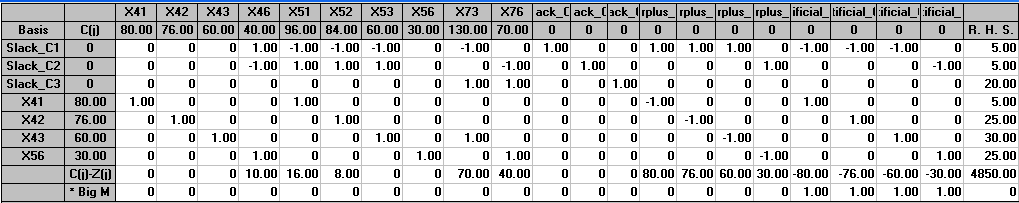
\includegraphics[width=\textwidth]{res/Exercise_1_pp_simplex_final.png}
	        \end{figure}

			\paragraph{}
			Si nos fijamos en la última columna objervamos que los valores que consiguen el óptimo de la función objetivo son:
			\(x_{41}^{*} = 5 \), \(x_{42}^{*} = 25 \), \(x_{43}^{*} = 30 \), \(x_{56}^{*} = 25 \) lo cual resulta en \(z^{*} = 4850 \).

			\paragraph{}
			La traducción de este resultado nos indica que para que el empresario pueda tener al menos 100 cartuchos en cada una de sus tiendas tendrá que envíar:

			\begin{itemize}
				\item 5 cartuchos de la tienda 4 a la tienda 1.
				\item 25 cartuchos de la tienda 4 a la tienda 2.
				\item 30 cartuchos de la tienda 4 a la tienda 3.
				\item 25 cartuchos de la tienda 5 a la tienda 6.
			\end{itemize}

			Esto le ocasionará un coste de 4850 céntimos de euro, es decir, 48.50\euro

		\subsection{?`En cuánto puede variar el coste de envío entre las tiendas 4 y 6 para que la solución Óptima calculada en el apartado (a) se mantenga? Razonar la respuesta.}

			\paragraph{}


		\subsection{Sin realizar iteraciones, obtener la nueva solución si el número de cartuchos disponibles en la tienda número 3 disminuye a 65 y el de la tienda 5 aumenta a 135 unidades. Justificar la respuesta.}

			\paragraph{}


		\subsection{Escribir el problema dual del formulado en el apartado (a)}

			\paragraph{}


		\subsection{Resolver el problema del apartado (e) utilizando las condiciones de holgura complementaria. ?`Es única la solución? Razonar la respuesta.}

			\paragraph{}


		\subsection{Suponer ahora que los cartuchos se pueden enviar entre todas las tiendas conectadas. Modelizar, sin resolver, este nuevo problema.}

			\paragraph{}


    \section{Ejercicio 2}

        \begin{figure}[H]
        \centering
            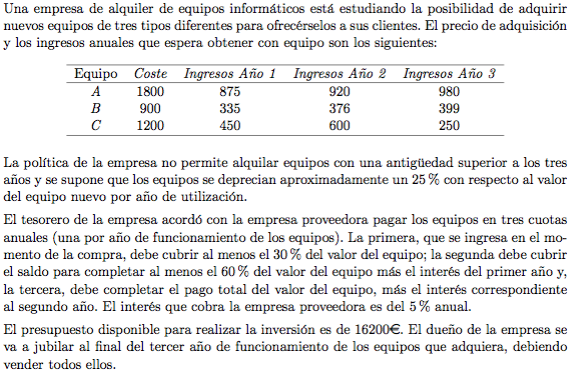
\includegraphics[width=0.75\textwidth]{res/Exercise_2.png}
        \end{figure}

		\subsection{Formular un modelo de PL para determinar el plan Óptimo de compras y de pagos que maximice los beneficios al final del periodo de tres años.}

			\paragraph{}


		\subsection{?`Cuál es el plan Óptimo?}

			\paragraph{}


		\subsection{Escribir el problema dual del formulado en el apartado (a).}

			\paragraph{}


		\subsection{Determinar la solución Óptima del problema formulado en (c) utilizando las condiciones de holgura complementaria.}

			\paragraph{}


		\subsection{Interpretar la variable dual asociada a la restricción del presupuesto disponible.}

			\paragraph{}


\end{document}
